% GNUPLOT: LaTeX picture with Postscript
\begingroup
  % Encoding inside the plot.  In the header of your document, this encoding
  % should to defined, e.g., by using
  % \usepackage[cp1252,<other encodings>]{inputenc}
  \inputencoding{cp1252}%
  \makeatletter
  \providecommand\color[2][]{%
    \GenericError{(gnuplot) \space\space\space\@spaces}{%
      Package color not loaded in conjunction with
      terminal option `colourtext'%
    }{See the gnuplot documentation for explanation.%
    }{Either use 'blacktext' in gnuplot or load the package
      color.sty in LaTeX.}%
    \renewcommand\color[2][]{}%
  }%
  \providecommand\includegraphics[2][]{%
    \GenericError{(gnuplot) \space\space\space\@spaces}{%
      Package graphicx or graphics not loaded%
    }{See the gnuplot documentation for explanation.%
    }{The gnuplot epslatex terminal needs graphicx.sty or graphics.sty.}%
    \renewcommand\includegraphics[2][]{}%
  }%
  \providecommand\rotatebox[2]{#2}%
  \@ifundefined{ifGPcolor}{%
    \newif\ifGPcolor
    \GPcolortrue
  }{}%
  \@ifundefined{ifGPblacktext}{%
    \newif\ifGPblacktext
    \GPblacktextfalse
  }{}%
  % define a \g@addto@macro without @ in the name:
  \let\gplgaddtomacro\g@addto@macro
  % define empty templates for all commands taking text:
  \gdef\gplbacktext{}%
  \gdef\gplfronttext{}%
  \makeatother
  \ifGPblacktext
    % no textcolor at all
    \def\colorrgb#1{}%
    \def\colorgray#1{}%
  \else
    % gray or color?
    \ifGPcolor
      \def\colorrgb#1{\color[rgb]{#1}}%
      \def\colorgray#1{\color[gray]{#1}}%
      \expandafter\def\csname LTw\endcsname{\color{white}}%
      \expandafter\def\csname LTb\endcsname{\color{black}}%
      \expandafter\def\csname LTa\endcsname{\color{black}}%
      \expandafter\def\csname LT0\endcsname{\color[rgb]{1,0,0}}%
      \expandafter\def\csname LT1\endcsname{\color[rgb]{0,1,0}}%
      \expandafter\def\csname LT2\endcsname{\color[rgb]{0,0,1}}%
      \expandafter\def\csname LT3\endcsname{\color[rgb]{1,0,1}}%
      \expandafter\def\csname LT4\endcsname{\color[rgb]{0,1,1}}%
      \expandafter\def\csname LT5\endcsname{\color[rgb]{1,1,0}}%
      \expandafter\def\csname LT6\endcsname{\color[rgb]{0,0,0}}%
      \expandafter\def\csname LT7\endcsname{\color[rgb]{1,0.3,0}}%
      \expandafter\def\csname LT8\endcsname{\color[rgb]{0.5,0.5,0.5}}%
    \else
      % gray
      \def\colorrgb#1{\color{black}}%
      \def\colorgray#1{\color[gray]{#1}}%
      \expandafter\def\csname LTw\endcsname{\color{white}}%
      \expandafter\def\csname LTb\endcsname{\color{black}}%
      \expandafter\def\csname LTa\endcsname{\color{black}}%
      \expandafter\def\csname LT0\endcsname{\color{black}}%
      \expandafter\def\csname LT1\endcsname{\color{black}}%
      \expandafter\def\csname LT2\endcsname{\color{black}}%
      \expandafter\def\csname LT3\endcsname{\color{black}}%
      \expandafter\def\csname LT4\endcsname{\color{black}}%
      \expandafter\def\csname LT5\endcsname{\color{black}}%
      \expandafter\def\csname LT6\endcsname{\color{black}}%
      \expandafter\def\csname LT7\endcsname{\color{black}}%
      \expandafter\def\csname LT8\endcsname{\color{black}}%
    \fi
  \fi
    \setlength{\unitlength}{0.0500bp}%
    \ifx\gptboxheight\undefined%
      \newlength{\gptboxheight}%
      \newlength{\gptboxwidth}%
      \newsavebox{\gptboxtext}%
    \fi%
    \setlength{\fboxrule}{0.5pt}%
    \setlength{\fboxsep}{1pt}%
    \definecolor{tbcol}{rgb}{1,1,1}%
\begin{picture}(5760.00,3772.00)%
    \gplgaddtomacro\gplbacktext{%
      \csname LTb\endcsname%%
      \put(1342,1274){\makebox(0,0){\scriptsize -0.008}}%
      \put(1342,1460){\makebox(0,0){\scriptsize -0.006}}%
      \put(1342,1646){\makebox(0,0){\scriptsize -0.004}}%
      \put(1342,1832){\makebox(0,0){\scriptsize -0.002}}%
      \put(1342,2018){\makebox(0,0){\scriptsize 0}}%
      \put(1342,2203){\makebox(0,0){\scriptsize 0.002}}%
      \put(1342,2389){\makebox(0,0){\scriptsize 0.004}}%
      \put(1342,2575){\makebox(0,0){\scriptsize 0.006}}%
      \put(1342,2761){\makebox(0,0){\scriptsize 0.008}}%
      \put(2016,1142){\makebox(0,0){\scriptsize 5}}%
      \put(2528,1142){\makebox(0,0){\scriptsize 10}}%
      \put(3041,1142){\makebox(0,0){\scriptsize 15}}%
      \put(3553,1142){\makebox(0,0){\scriptsize 20}}%
      \put(4066,1142){\makebox(0,0){\scriptsize 25}}%
      \put(4578,1142){\makebox(0,0){\scriptsize 30}}%
      \put(3092,2850){\makebox(0,0){\strut{}SC}}%
    }%
    \gplgaddtomacro\gplfronttext{%
      \csname LTb\endcsname%%
      \put(4747,3364){\makebox(0,0)[l]{\strut{}\footnotesize 1}}%
      \csname LTb\endcsname%%
      \put(4747,3144){\makebox(0,0)[l]{\strut{}\footnotesize 2}}%
      \csname LTb\endcsname%%
      \put(4747,2924){\makebox(0,0)[l]{\strut{}\footnotesize 3}}%
      \csname LTb\endcsname%%
      \put(4747,2704){\makebox(0,0)[l]{\strut{}\footnotesize 4}}%
      \csname LTb\endcsname%%
      \put(4747,2484){\makebox(0,0)[l]{\strut{}\footnotesize 5}}%
      \csname LTb\endcsname%%
      \put(4747,2264){\makebox(0,0)[l]{\strut{}\footnotesize 6}}%
      \csname LTb\endcsname%%
      \put(4747,2044){\makebox(0,0)[l]{\strut{}\footnotesize 7}}%
      \csname LTb\endcsname%%
      \put(4747,1824){\makebox(0,0)[l]{\strut{}\footnotesize 8}}%
      \csname LTb\endcsname%%
      \put(4747,1604){\makebox(0,0)[l]{\strut{}\footnotesize 9}}%
      \csname LTb\endcsname%%
      \put(4747,1384){\makebox(0,0)[l]{\strut{}\footnotesize 10}}%
      \csname LTb\endcsname%%
      \put(6130,3364){\makebox(0,0)[l]{\strut{}\footnotesize 11}}%
      \csname LTb\endcsname%%
      \put(6130,3144){\makebox(0,0)[l]{\strut{}\footnotesize 12}}%
      \csname LTb\endcsname%%
      \put(6130,2924){\makebox(0,0)[l]{\strut{}\footnotesize 13}}%
      \csname LTb\endcsname%%
      \put(6130,2704){\makebox(0,0)[l]{\strut{}\footnotesize 14}}%
      \csname LTb\endcsname%%
      \put(6130,2484){\makebox(0,0)[l]{\strut{}\footnotesize 15}}%
      \csname LTb\endcsname%%
      \put(6130,2264){\makebox(0,0)[l]{\strut{}\footnotesize 16}}%
      \csname LTb\endcsname%%
      \put(6130,2044){\makebox(0,0)[l]{\strut{}\footnotesize 17}}%
      \csname LTb\endcsname%%
      \put(6130,1824){\makebox(0,0)[l]{\strut{}\footnotesize 18}}%
      \csname LTb\endcsname%%
      \put(6130,1604){\makebox(0,0)[l]{\strut{}\footnotesize 19}}%
      \csname LTb\endcsname%%
      \put(6130,1384){\makebox(0,0)[l]{\strut{}\footnotesize 20}}%
      \csname LTb\endcsname%%
      \put(869,2017){\rotatebox{-270.00}{\makebox(0,0){\strut{}$\bm{Re(\Delta)$}}}}%
      \put(3092,944){\makebox(0,0){\small\textbf{Lattice site $i$ in $\bm{e}_x$}}}%
      \put(4932,1274){\makebox(0,0)[l]{\strut{}$-10$}}%
      \put(4932,1645){\makebox(0,0)[l]{\strut{}$-5$}}%
      \put(4932,2017){\makebox(0,0)[l]{\strut{}$0$}}%
      \put(4932,2389){\makebox(0,0)[l]{\strut{}$5$}}%
      \put(4932,2761){\makebox(0,0)[l]{\strut{}$10$}}%
    }%
    \gplbacktext
    \put(0,0){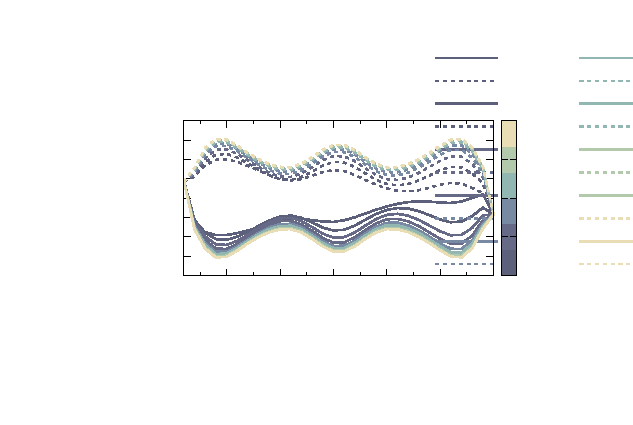
\includegraphics[width={288.00bp},height={188.60bp}]{Plots/SC30/MeanLine_Phase/Phase117deg/mu/LinearGradient/long-3.75/plot}}%
    \gplfronttext
  \end{picture}%
\endgroup

